\documentclass{standalone}
\usepackage{amsmath}
\usepackage{amsfonts}
\usepackage{amssymb}
\usepackage{tikz}
\usetikzlibrary{positioning}
\usetikzlibrary{decorations.pathreplacing}
\usetikzlibrary{decorations.text}
\usetikzlibrary{arrows,shapes,backgrounds, shadows,fadings}
\usetikzlibrary{calc, intersections}
\usepackage{color}
\definecolor{ColorA}{rgb}{0.1,0.2,0.5}
\definecolor{ColorB}{rgb}{0.2,0.45,0.15}




\begin{document}
	
	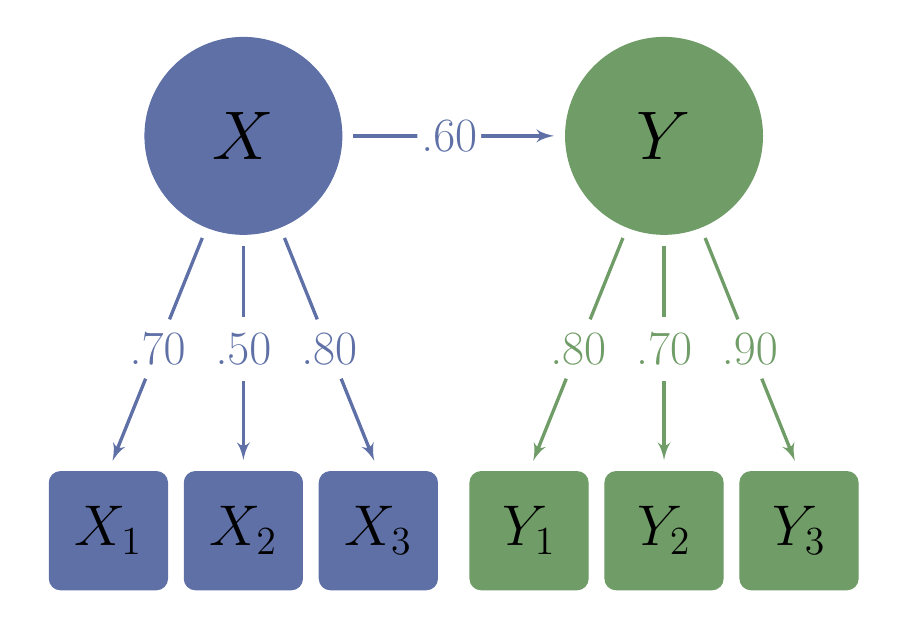
\begin{tikzpicture}[latent/.style={circle, minimum size=2.5cm,inner sep=0cm,font=\Huge},
	error/.style={circle,inner sep=0mm, minimum size=0.85cm,font=\large},
	ob/.style={rectangle,inner sep=1mm, minimum width=1.5cm, minimum height=1.5cm, rounded corners,font=\huge},
	post/.style={->,draw,shorten >=4pt,shorten <=4pt,>=latex', very thick},
	cov/.style={<->,draw,shorten >=4pt,shorten <=4pt,>=latex', very thick, font=\large, bend left=50},
	variance/.style={<->,  >=latex', thick, bend left=245, looseness=5,shorten >=2pt,shorten <=2pt, draw = black},
	label/.style={fill=white,circle,inner sep = 0mm, font = \LARGE},
	tri/.style = {regular polygon, regular polygon sides=3,
		text width=1em, font = \Large,
		inner sep=1.1mm, outer sep=0mm,align=center},
	A/.style = {fill=ColorA!70,draw = ColorA!70},
	B/.style = {fill=ColorB!70,draw = ColorB!70},
	C/.style = {fill=ColorC!50,draw = ColorC!50}]
	
	% Observed
	\node[ob, A] (A1) at (0,0) {$X_1$};
	\node[ob, A, right = 0.2cm of A1] (A2) {$X_2$};
	\node[ob, A, right = 0.2cm of A2] (A3) {$X_3$};
	\node[ob, B, right = 0.4cm of A3] (B1) {$Y_1$};
	\node[ob, B, right = 0.2cm of B1] (B2) {$Y_2$};
	\node[ob, B, right = 0.2cm of B2] (B3) {$Y_3$};
	% Latent
	\node[latent, A, above = 3cm of A2.north] (A) {$X$};
	\node[latent, B, above = 3cm of B2.north] (B) {$Y$};
	
	\coordinate[left = 1.5cm of A1.north, yshift = 1.55cm] (x0);
	\coordinate[right = 1.5cm of B3.north, yshift = 1.55cm] (x6);

	
	\path[post, A] (A) to (A1.north);
	\path[post, A] (A) to (A2.north);
	\path[post, A] (A) to (A3.north);
	
	\path[post, B] (B) to (B1.north);
	\path[post, B] (B) to (B2.north);
	\path[post, B] (B) to (B3.north);

	\path[post, A] (A) to node[label, text = ColorA!70, pos = 0.48] {.60} (B);

	
	\node[label, text = ColorA!70] (E) at (intersection of A--A1.north and x0--x6) {.70};
	\node[label, text = ColorA!70] (E) at (intersection of A--A2.north and x0--x6) {.50};
	\node[label, text = ColorA!70] (E) at (intersection of A--A3.north and x0--x6) {.80};
	
	\node[label, text = ColorB!70] (E) at (intersection of B--B1.north and x0--x6) {.80};
	\node[label, text = ColorB!70] (E) at (intersection of B--B2.north and x0--x6) {.70};
	\node[label, text = ColorB!70] (E) at (intersection of B--B3.north and x0--x6) {.90};
	
	
	
	
	\node[xshift = -1ex] at (current bounding box.south west){};
	\node[xshift = 1ex] at (current bounding box.north east){};
	\end{tikzpicture}
	
\end{document}

